\documentclass[12pt,a4paper]{scrartcl} 

%Deutsch:
	\usepackage[ngerman]{babel} %Deutsches Datumformat, Umlaute m\"oglich,...
	\usepackage[utf8]{inputenc}
	\usepackage[T1]{fontenc} 
	
%Quellenverzeichnis:
	\usepackage[maxcitenames=2,autocite=footnote,uniquename=full,uniquelist=true,backend=biber]{biblatex} %style=authoryear-icomp
	\usepackage{csquotes} %Hilfspaket für Biblatex
	\bibliography{bib_database.bib} %Datei mit bibliographischen Daten
	\DefineBibliographyStrings{ngerman}{andothers={et\ al\adddot}} % "u.a." zu "et al."
	\DefineBibliographyStrings{ngerman}{and={\&}} % "und" zu "&"

%Mathematik:
	\usepackage{dsfont} %Symbole
	\usepackage{amsmath} %Umgebung
	\usepackage{amssymb} %Symbole
	\usepackage{bbm} %doppelstreifen bei buchstaben (zb symbol für ganze zahlen \mathbbm{Z})
	
%Grafiken:
	\usepackage{graphics}
	\usepackage{graphicx}
	\usepackage{picinpar} %bilder so einfügen, dass text um bilder weiterläuft
	\usepackage{float} %\begin{figure}[H] => Grafik wird HIER eingefügt!

%Euro-Zeichen:
	\usepackage{eurosym}

%Quellcode:
	%\usepackage[numbered,framed]{mcode} %Quellcode darstellen
	
%Englisch:
	%\usepackage[ngerman,english]{babel} %automatisch erzeugte Überschriften etc. auf englisch
	
\DeclareMathOperator*{\argmin}{arg\,min} % Importiere die Einstellungen aus der Pr?ambel

%%%%%%%%%%%%%%%%%%%%%%%%%%%%%%%%%%%%%%%%%%%%%%%%%%%%%%%%%%
% hier kommen die packages für Latex hin, falls sie nicht schon wo anders geladen werden
% \usepackage{amssymb}
% \usepackage{graphicx}
% \usepackage[utf8]{inputenc}
% \usepackage[ngerman]{babel}
% \usepackage{tikz}
%%%%%%%%%%%%%%%%%%%%%%%%%%%%%%%%%%%%%%%%%%%%%%%%%%%%%%%%%%


%%%%%%%%%%%%%%%%%%%%%%%%%%%%%%%%%%%%%%%%%%%%%%%%%%%%%%%%%%
% Hier können die Pakete, die benötigten Daten und Graphen für R geladen bzw erstellt werden.
% echo=FALSE gibt keinen R Output wieder

%%%%%%%%%%%%%%%%%%%%%%%%%%%%%%%%%%%%%%%%%%%%%%%%%%%%%%%%%%


% hier beginnt der eigentliche Inhalt
\usepackage{Sweave}
\begin{document}
\Sconcordance{concordance:Bericht_Sweave.tex:Bericht_Sweave.Rnw:%
1 15 1 1 7 5 1 1 0 28 1 2 2 7 1}


% Deckblatt
\begin{titlepage}
	\rmfamily
	\begin{center}
		% Logo
		%\includegraphics[width=0.15\textwidth]{./logo}\\[1cm]
	
		\textsc{\LARGE Statistisches Consulting}\\[1.5cm]

		\textsc{
			\large{	Master Studiengang Statistik\\[0.25cm]
							Institut für Statistik\\[0.25cm]
							Ludwig-Maximilians-Universität München}}\\[0.25cm]
						
		% Title
		\newcommand{\HRule}{\rule{\linewidth}{0.5mm}}
		\HRule \\[0.4cm]
		{\huge \bfseries Online-Marketing der Interhyp AG\\[0.5cm]Analyse von Tracking-Daten}\\[0.4cm]
		\HRule \\[1.5cm]
		
		% Autoren
		\textbf{Daniel Fuckner} d.fuckner@gmx.de\\
		\textbf{Markus Vogler} markus@vogler-lindau.de\\[1.5cm]
	
		% Betreuer und Projektpartner
		\begin{minipage}{0.4\textwidth}
			\begin{flushleft}
				Projektpartner:\\
				\textbf{Interhyp AG}
			\end{flushleft}
		\end{minipage}
		\hfill
		\begin{minipage}{0.4\textwidth}
			\begin{flushright}
				Betreuer:\\
				\textbf{Dr. Fabian Scheipl}
			\end{flushright}
		\end{minipage}
		
		\vfill

		% Datum
		{\large München, 11.11.2011}
		
	\end{center}
\end{titlepage}

%\thispagestyle{plain}
\pagenumbering{roman} %r?mische Seitennummerierung

%Abstract
\begin{abstract}
  \noindent
	\paragraph{Abstract:}
	\paragraph{Background:} In patients with
\end{abstract}

%Inhaltsverzeichnis
\newpage
\tableofcontents

\newpage
\pagenumbering{arabic} %ab hier wieder normale Seitennummerierung

% Hier beginnt der eigentliche Text
\section{abc}
asdfsadf \cite[186]{taxonomy}
\subsection{abcd} % Importiere die Einleitung

Ab hier kann man dann wieder normal schreiben.Sweave test mit chunk1\\


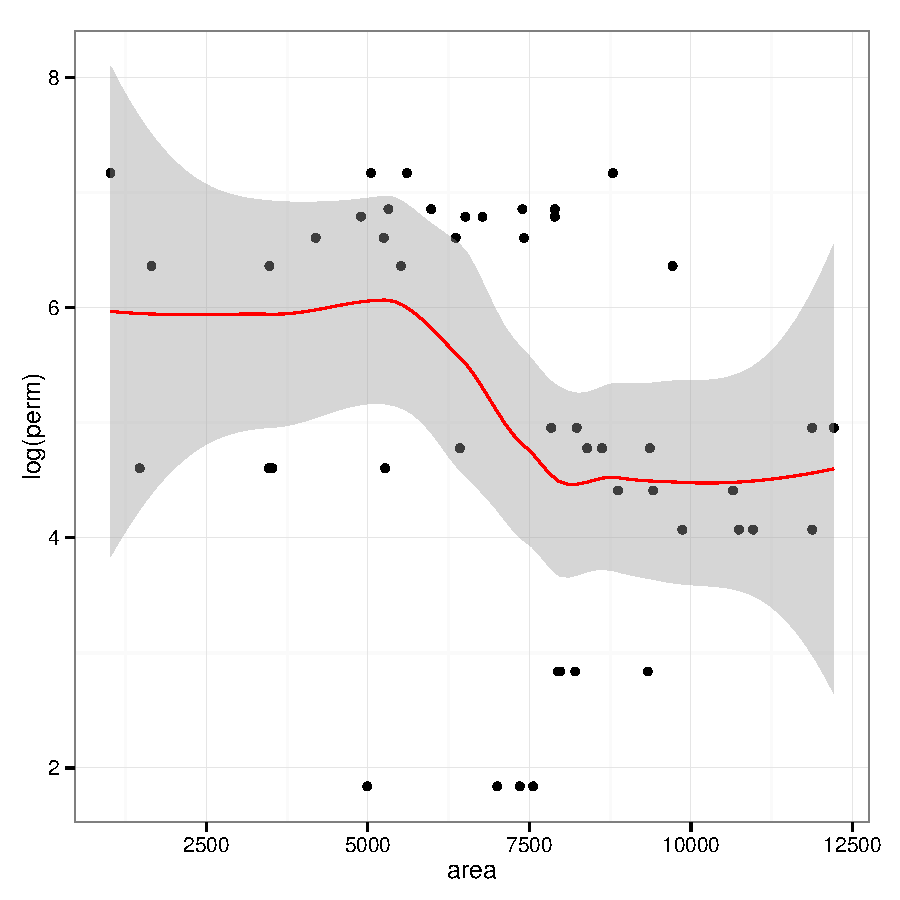
\includegraphics{Bericht_Sweave-002}



%Literaturverzeichnis
\newpage
\printbibliography 

\end{document}
